
The impact of the signal efficiency systematic uncertainty on the expected limit is studied. 
The luminosity and background predictions together with their uncertainties are fixed to the ones used 
in this analysis, while the signal efficiency and its relative uncertainty are varied.


\begin{figure}[htbp]
\centering
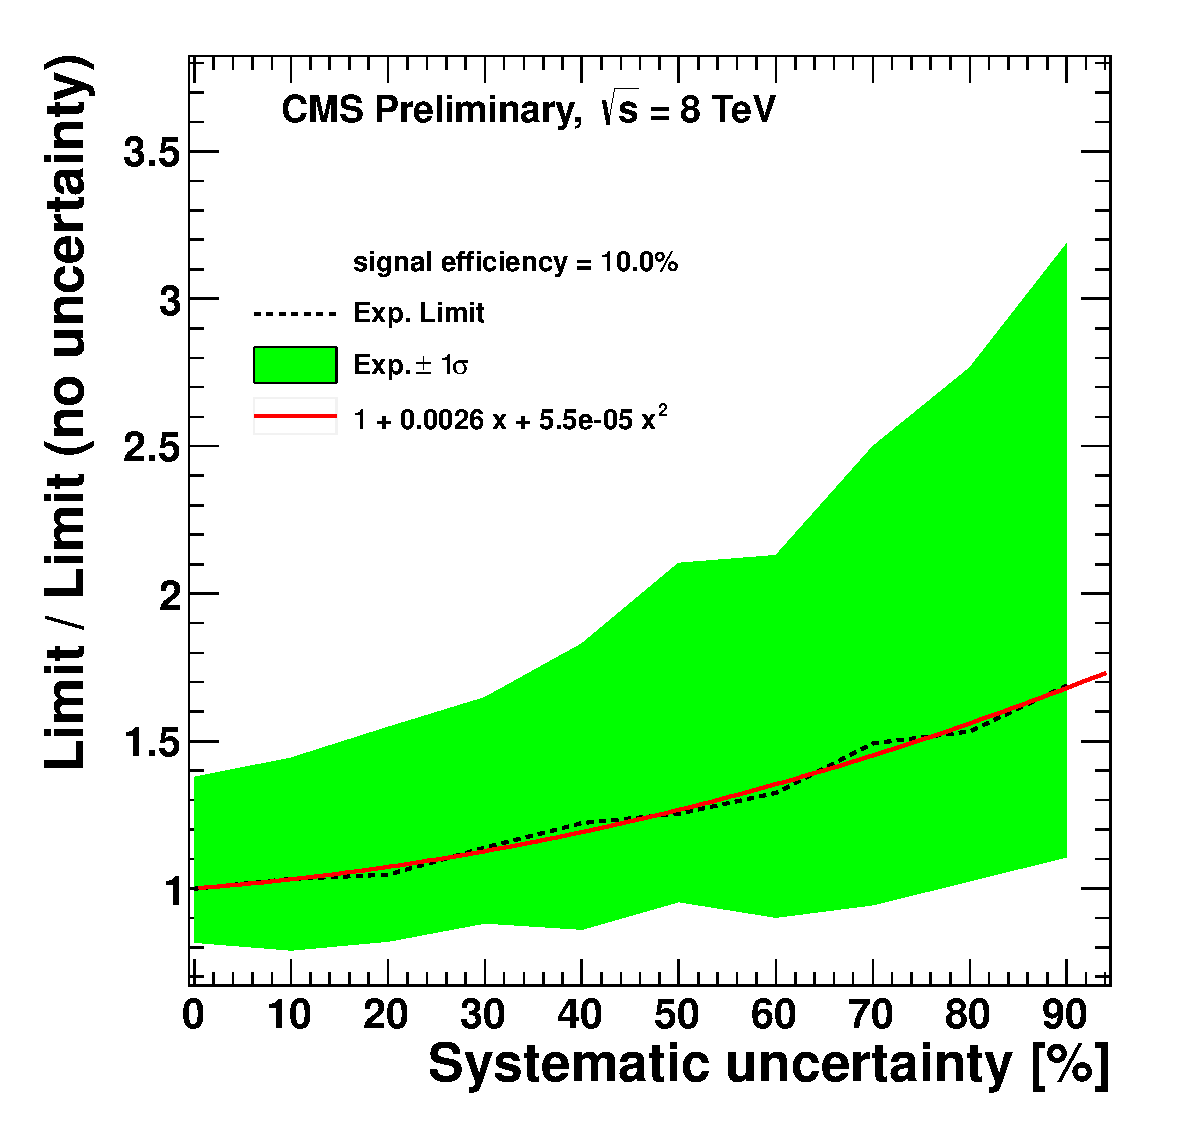
\includegraphics[width=0.45\textwidth]{plots/degradation/10percent.pdf}
\includegraphics[width=0.45\textwidth]{plots/degradation/1percent.pdf}
\caption{Expected limit degradation as a function of signal efficiency systematic uncertainty.
The signal efficiency central value is assumed to be 10\% (left) and 1\% (right). A second order polynomial
is fitted to the expected limit graph with the fit parameter values listed in the legend.\label{fig:degradation}}
\end{figure}

Figure \ref{fig:degradation} shows the relative expected limit and 1$\sigma$ band degradation as the 
systematic uncertainty on signal efficiency is varied from 0 to 90\%. The degradation of the limit does not depend
on the central value of the efficiency itself. Relative to a limit obtained with no uncertainty, a 
degradation of 10\% is observed for a 30\% the systematic uncertainty. The limit degradation has also been studied 
assuming Gaussian or Log-normal parametrizations of the nuisance parameters yielding similar results.

In this analysis the systematic uncertainty on the signal efficiency has been conservatively 
estimated to at most 10\% for all signal models considered. A precise estimate of its value is of secondary importance given a small impact on the resulting limit.
      

